\chapter{Identifikasi Masalah dan Rancangan Solusi}

Bab Identifikasi Masalah dan Rancangan Solusi berisi tentang penjelasan analisis permasalahan yang menjadi dasar dari tugas akhir ini. Secara garis besar, proses perancangan solusi akan mengikuti metodologi yang sudah ditetapkan yaitu pendekatan \textit{User-Centered Design} (UCD) menurut ISO 9241-210. Proses yang akan dibahas pada bab ini meliputi perancangan proses desain, identifikasi konteks penggunaan, analisis kebutuhan perangkat lunak, dan perancangan prototipe perangkat lunak. Gambaran alur UCD yang digunakan pada tugas akhir dapat dilihat pada Gambar \ref{fig:diagram_alur_kerja}.

\begin{figure}[h]
  \centering
  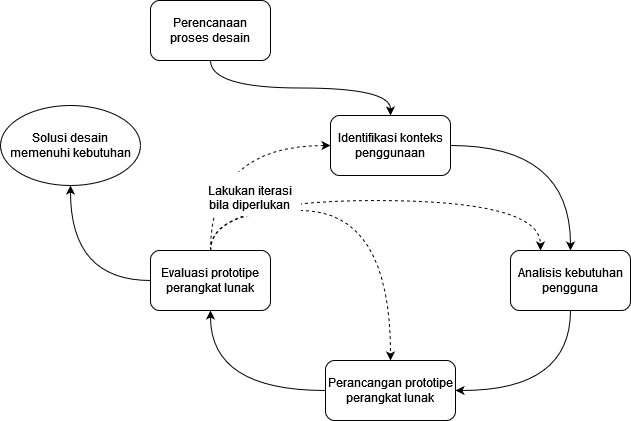
\includegraphics[width=0.8\textwidth]{chapter-1-method.png}
  \caption{Alur Kerja Penelitian}
  \label{fig:diagram_alur_kerja}
\end{figure}

\section{Perancangan Proses Desain}
\label{sec:perancangan_proses_desain}

Pada tahap perancangan proses desain dilakukan persiapan sumber daya yang diperlukan selama proses desain, serta penentuan ruang lingkup permasalahan.

Adapun ruang lingkup permasalahan yang ditentukan selama pengerjaan tugas akhir sebagai berikut

\begin{enumerate}
  \item Target Pengguna
  \subitem Target pengguna selama penelitian adalah pengguna \textit{smartphone} berbasis Android di Indonesia dengan rentang umur 18-34 tahun. Rentang usia tersebut adalah usia mayoritas pengguna media sosial di Indonesia. \parencite{mediasosial2020} 
  
  \item Fungsionalitas Aplikasi
  \subitem Lingkup fungsionalitas aplikasi adalah bagaimana desain interaksi yang baru dapat memperbaiki masalah yang ditemukan pada aplikasi Digital Wellbeing saat ini. Fungsionalitas dar aplikasi menyesuaikan dengan analisis hasil yang didapatkan dari riset dan wawancara. 
   
  \item Lingkup Pengembangan Aplikasi
  \subitem Desain interaksi aplikasi pencegah distraksi yang dibuat memiliki bentuk \textit{mobile interface} dengan mewujudkan sebuah prototipe aplikasi dalam \textit{platform Android}. Aplikasi Digital Wellbeing milik Google ditetapkan menjadi garis dasar pengembangan prototipe aplikasi tersebut.

\end{enumerate}

% \subsection{Sumber Daya Proses Desain}

\section{Identifikasi Konteks Penggunaan}
\label{sec:identifikasi_konteks_penggunaan}

Pada tahap ini dilakukan proses analisis pengguna melalui data yang didapatkan dari ulasan pengguna aplikasi Digital Wellbeing dari situs Google Play Store, serta riset dengan metode wawancara.
% Hasil analisis pengguna digunakan untuk menyusun kebutuhan fungsional 

\subsection{Riset dan Analisis Pengguna}

Tahap ini bertujuan untuk menganalis target pengguna, sehingga didapatkan data perilaku, masalah, tujuan, dan kebutuhan pengguna aplikasi Digital Wellbeing. Riset dilakukan dengan mengumpulkan data ulasan pengguna aplikasi Digital Wellbeing dari situs Google Play Store \textcite{dwplaystorereviews}. Metode pengumpulan data ini dipilih dengan alasan mengacu pada ISO 9241-210, bahwa informasi yang sudah tersedia dari suatu produk dapat dimanfaatkan untuk melakukan modifikasi atau peningkatan kualitas produk \parencite{iso9241-210:2010}, dalam hal ini informasi berbentuk ulasan pengguna.

Berdasarkan situs Google Play Store per 13 April 2022, terdapat 609.005 ulasan untuk aplikasi Digital Wellbeing. Untuk menentukan jumlah \textit{sample size}, ditentukan \textit{confidence level} sebesar 95\%. Dikumpulkan data sebanyak 1000 ulasan dari target pengguna yang telah disebutkan pada bab \ref{sec:identifikasi_konteks_penggunaan},  kemudian dikategorikan secara manual, lalu didapatkan 291 ulasan yang dapat digunakan untuk menyusun masalah pengguna, sehingga \textit{sample} data memiliki \textit{margin of error} sebesar 5.75\%.

Metode pengkategorian ulasan menjadi daftar masalah pengguna dilakukan secara manual yang menghasilkan 12 kategori masalah. Rincian tentang kategori tersebut dapat dilihat pada tabel \ref{tab:daftar_kategori}.

\begin{longtable}[c]{|p{0.07\textwidth}|p{0.75\textwidth}|p{0.09\textwidth}|}
  \caption{Daftar Kategori Ulasan Masalah}
  \label{tab:daftar_kategori} \\
  \hline ID & Kategori Masalah & Jumlah Ulasan \\ \hline \endfirsthead
  \hline ID & Kategori Masalah & Jumlah Ulasan \\ \hline \endhead

  \hline \endfoot

  K-01    & Kurangnya widget untuk menampilkan data di Home Screen & 63 \\ \hline
  K-02    & Perlu dikembangkannya fitur laporan penggunaan aplikasi & 47 \\ \hline
  K-03    & Perlu dikembangkannya fitur Focus Mode & 47 \\ \hline
  K-04    & Kurangnya fitur pengaturan tingkat ketetatan & 29 \\ \hline
  K-05    & Kurangnya fitur penjadwalan terhadap akses aplikasi & 19 \\ \hline
  K-06    & Kurangnya fitur penunda batas waktu penggunaan aplikasi & 18 \\ \hline
  K-07    & Perlu dibedakannya pengaturan untuk akhir pekan & 17 \\ \hline
  K-08    & Kurangnya penjelasan untuk deskripsi fitur & 12 \\ \hline
  K-09    & Perlu dikembangkannya fitur Bedtime Mode & 12 \\ \hline
  K-10    & Kurangnya fitur kategorisasi aplikasi & 11 \\ \hline
  K-11    & Kurangnya fitur pengaturan jam akhir sebuah hari & 7 \\ \hline
  K-12    & Kurangnya fitur \textit{whitelisting} untuk pembatasan akses aplikasi & 6 \\ \hline
\end{longtable}

\FloatBarrier

Adapun ulasan yang tidak tergolong dalam kategori dinilai tidak relevan dalam penyusunan masalah pengguna, dengan penjelasan sebagai berikut

\begin{enumerate}
  \item Ulasan yang menilai positif aplikasi tanpa menyebutkan adanya masalah yang ditemukan dari aplikasi
  \item Ulasan yang menilai negatif aplikasi tanpa menyebutkan masalah yang ditemukan dari aplikasi
  \item Ulasan yang menyebutkan adanya bug dari aplikasi, seperti tidak berfungsinya sebuah fitur di perangkat tertentu
  \item Ulasan yang menyebutkan masalah yang tidak termasuk ke dalam batasan tugas akhir
  \item Ulasan yang tidak dapat dimengerti, seperti huruf-huruf yang tersusun secara acak 
\end{enumerate}

Data yang terkumpul berjumlah 1000 ulasan yang berasal dari \textit{region} Indonesia, sesuai dengan target pengguna yang telah disebutkan pada bab \ref{sec:perancangan_proses_desain}. Data tersebut kemudian dikategorikan berdasarkan masalah yang dilaporkan 
dengan bantuan library Python. Keterangan proses dan hasil pengumpulan data dapat dilihat pada Lampiran \ref{chpt:web_scraping}. 

% \begin{table}[t]
%   \centering
%   \fontsize{10}{12}
%   \caption{Daftar Permasalahan}
%   \label{tab:daftar_permasalahan}
%   \vspace{0.2cm}
%   \begin{tabular}{|p{0.12\textwidth}|p{0.81\textwidth}|}
%   \hline
%   ID    & Masalah Aplikasi Digital Wellbeing \\ \hline
%   M-01    & Fitur-fitur pada aplikasi Digital Wellbeing kurang dapat membatasi akses pengguna dengan cukup ketat \\ \hline
%   M-02    & Fitur-fitur pada aplikasi Digital Wellbeing kurang memberikan fleksibilitas dalam menunda pembatasan akses pengguna \\ \hline
%   M-03    & Aplikasi Digital Wellbeing kurang memberikan fleksibilitas bagi pengguna dalam mengatur jadwal aktivasi fitur \\ \hline
%   M-04    & Aplikasi Digital Wellbeing tidak dapat mengelompokkan aplikasi berdasarkan kategori yang ditentukan oleh pengguna \\ \hline
%   M-05    & Aplikasi Digital Wellbeing kurang memberikan laporan yang komprehensif tentang aktivitas pengguna \textit{smartphone} \\ \hline
%   M-06    & Aplikasi Digital Wellbeing saat ini hanya memiliki 1 buah \textit{widget} yang dapat menampilkan total \textit{screentime} pengguna \textit{smartphone} dan 3 aplikasi dengan penggunaan tertinggi di hari tersebut\\ \hline
%   \end{tabular}
% \end{table}

Sebagai batasan masalah, perlu disebutkan bahwa tidak adanya kemampuan untuk menghapus aplikasi Digital Wellbeing dari perangkat tidak akan dijadikan rumusan masalah, hal ini memiliki alasan yaitu menghapus aplikasi dari perangkat bukanlah solusi yang sejajar dengan masalah yang ingin diselesaikan dari konsep Digital Wellbeing. Selain itu, masalah yang berhubungan dengan performa aplikasi atau dampaknya pada perangkat tidak akan dijadikan rumusan masalah, namun saat pembangunan solusi hal ini akan diperhatikan agar tidak mengganggu tahap pengujian.


% \section{Analisis Solusi}
% \label{sec:analisis_solusi}

% Dari permasalahan yang telah diuraikan pada subbab \ref{sec:analisis_masalah}, terdapat beberapa solusi yang dapat diimplementasikan ke dalam aplikasi pencegah distraksi untuk mencapai tujuan dari aplikasi Digital Wellbeing dengan lebih baik yaitu menghambat akses pengguna terhadap aplikasi distraksi secara efektif dan memotivasi pengguna untuk mengubah pola penggunaan aplikasi secara general. Setiap solusi akan dijelaskan tentang permasalahan apa yang akan diselesaikan. Solusi yang ditawarkan untuk menyelesaikan masalah yang telah dianalisis dicantumkan pada Tabel \ref{tab:daftar_solusi}. Rincian mengenai solusi tersebut dapat dilihat pada Lampiran \ref{chpt:rincian_analisis_solusi}.

Berdasarkan hasil analisis permasalahan yang dilakukan, maka solusi yang akan dibuat adalah sebuah prototipe aplikasi pencegah distraksi dengan tampilan mendekati aplikasi Digital Wellbeing yang dapat menyelesaikan rumusan masalah yang telah disebutkan pada Tabel \ref{tab:daftar_permasalahan}. Pada Tabel \ref{tab:daftar_solusi} terdapat pemetaan rumusan masalah kepada rancangan solusi dalam bentuk kebutuhan fungsional dan kebutuhan interaksi yang akan dimiliki oleh prototipe aplikasi

% \singlespacing
% >{\setlength{\baselineskip}{0.75\baselineskip}}p{0.17\linewidth}
\begin{longtable}[c]{|p{0.07\textwidth}|p{0.3\textwidth}|p{0.4\textwidth}|p{0.1\textwidth}|}
  % \centering
  % \fontsize{10}{12}
  \caption{Daftar Solusi}
  \label{tab:daftar_solusi} \\
  
  \hline
  ID  & Kebutuhan Fungsional & Kebutuhan Interaksi & Kode Masalah \\ \hline \endfirsthead

  \hline
  ID  & Kebutuhan Fungsional & Kebutuhan Interaksi & Kode Masalah \\ \hline \endhead

  \hline \endfoot

  S-01
  & \multirow{2}{0.3\textwidth}{Prototipe aplikasi dapat membatasi akses pengguna dengan cukup ketat}
  & Pengguna dapat memanfaatkan fitur "Take a break" pada Focus Mode hanya sebanyak waktu yang ditentukan per harinya
  & \multirow{4}{0.1\textwidth}{M-01} \\ \cline{1-1} \cline{3-3}
  
  S-02 &  
  & Pengguna perlu membuka kunci saat melakukan pengaturan pada fitur Focus Mode
  & \\ \cline{1-1} \cline{3-3}
  
  S-03 &  
  & Pengguna dapat memilih untuk menghilangkan kemampuan mematikan Focus Mode selama fitur berjalan
  & \\ \cline{1-1} \cline{3-3}
  
  S-04 &  
  & Pengguna perlu membuka kunci saat melakukan pengaturan pada fitur App Timer
  & \\ \cline{1-1} \cline{3-3}
  
  S-05 &  
  & Pengguna dapat membatasi aplikasi yang dapat diakses saat menggunakan fitur Bedtime Mode
  & \\ \cline{1-1} \cline{3-3}
  
  S-06 &  
  & Pengguna dapat menunda fitur Bedtime Mode hanya sebanyak waktu yang ditentukan per harinya
  
  & \\ \hline
  % ===========================
  S-07
  & \multirow{3}{0.3\textwidth}{Prototipe aplikasi dapat memberikan fleksibilitas dalam menunda pembatasan akses pengguna}
  & Pengguna dapat diingatkan terhadap batas App Timer beberapa saat lebih lama
  & \multirow{2}{0.1\textwidth}{M-02} \\ \cline{1-1} \cline{3-3}
  
  S-08 &  
  & Pengguna dapat diberikan tampilan durasi penggunaan aplikasi yang terdaftar dalam App Timer pada \textit{notification bar}
  & \\ \cline{1-1} \cline{3-3}
  
  S-09 &  
  & Pengguna dapat mengambil waktu tambahan yang terbatas untuk menggunakan aplikasi yang terdaftar dalam App Timer
  
  & \\ \hline
  % ===========================
  S-10
  & \multirow{2}{0.3\textwidth}{Prototipe dapat memberikan fleksibilitas bagi
  pengguna dalam mengatur jadwal aktivasi fitur}
  & Pengguna dapat membuat lebih dari 1 jadwal per minggu untuk fitur Focus Mode
  & \multirow{4}{0.1\textwidth}{M-03} \\ \cline{1-1} \cline{3-3}
  
  S-11 &  
  & Pengguna dapat menentukan waktu istirahat pada saat membuat jadwal untuk fitur Focus Mode
  & \\ \cline{1-1} \cline{3-3}
  
  S-12 &  
  & Pengguna dapat memilih membuat jadwal untuk membuka akses atau membatasi akses terhadap aplikasi untuk fitur Focus Mode   
  & \\ \cline{1-1} \cline{3-3}
  
  S-13 &  
  & Pengguna dapat mengatur waktu akhir hari untuk App Timer dan pelacakan data penggunaan harian  
  & \\ \cline{1-1} \cline{3-3}
  
  S-14 &  
  & Pengguna dapat membuat lebih dari 1 jadwal per minggu untuk fitur App Timer   
  & \\ \cline{1-1} \cline{3-3}
  
  S-15 &  
  & Pengguna dapat memilih membuat jadwal untuk membuka akses atau membatasi akses terhadap aplikasi untuk fitur App Timer   
  & \\ \cline{1-1} \cline{3-3}
  
  S-16 &  
  & Pengguna dapat membuat jadwal batas penggunaan per minggu untuk fitur App Timer   
  % & \\ \cline{1-1} \cline{3-3}

  & \\ \hline
  % ===========================
  S-17
  & Prototipe aplikasi dapat mengelompokkan aplikasi berdasarkan kategori yang ditentukan oleh pengguna
  & Pengguna dapat mengelompokkan aplikasi berdasarkan kategori yang ditentukan pengguna
  & M-04 \\ \hline
  
  % ===========================
  S-18
  & \multirow{3}{0.3\textwidth}{Prototipe aplikasi dapat memberikan laporan yang komprehensif tentang aktivitas pengguna smartphone}
  & Pengguna dapat melihat data waktu Focus Mode yang ditempuh
  & \multirow{2}{0.1\textwidth}{M-05} \\ \cline{1-1} \cline{3-3}

  S-19 &  
  & Pengguna dapat melihat laporan data rata-rata penggunaan \textit{smartphone} harian per minggu 
  & \\ \cline{1-1} \cline{3-3}

  S-20 &  
  & Pengguna dapat melihat laporan data rata-rata penggunaan aplikasi harian per minggu 
  & \\ \cline{1-1} \cline{3-3}

  S-21 &  
  & Pengguna dapat melihat laporan aktivitas lebih dari 10 hari yang lalu
  & \\ \cline{1-1} \cline{3-3}

  S-22 &  
  & Pengguna dapat melihat laporan aktivitas dengan periode waktu per bulan dan per tahun 
  & \\ \cline{1-1} \cline{3-3}

  & \\ \hline
  % ===========================
  S-23
  & \multirow{2}{0.3\textwidth}{Prototipe dapat memberikan fleksibilitas bagi
  pengguna dalam mengatur jadwal aktivasi fitur}
  & Pengguna dapat membuat lebih dari 1 jadwal per minggu untuk fitur Focus Mode
  & \multirow{4}{0.1\textwidth}{M-03} \\ \cline{1-1} \cline{3-3}

\end{longtable}

\FloatBarrier
% \onehalfspacing

Rancangan solusi yang dibuat akan divalidasi kepada pengguna aplikasi Digital Wellbeing dan sejenisnya sehingga dapat dibuat menjadi rancangan solusi yang sesuai dengan kebutuhan pengguna. Validasi akan dilakukan bersamaan dengan pengumpulan informasi pengguna, dan pengumpulan masalah lain dengan metode penyebaran kuesioner. Pertanyaan di dalam kuesioner didesain untuk mendapatkan informasi mengenai kebiasaan pengguna, masalah yang dialami pengguna saat ini, hingga kebutuhan pengguna.

\subsection{Riset dan Analisis Wawancara Pengguna}


% \blindtext

\section{Analisis Kebutuhan Perangkat Lunak}

% Proses perancangan solusi mengacu kepada metode \textit{User-Centered Design} sesuai dengan standar ISO 9241-210, di mana pada tahap perancangan desain interaksi untuk memenuhi kebutuhan pengguna akan disertai dengan prototipe aplikasi. Gambar \ref{fig:diagram_alur_kerja} menjelaskan tentang alur kerja penelitian yang dilakukan.

% \begin{figure}[h]
%   \centering
%   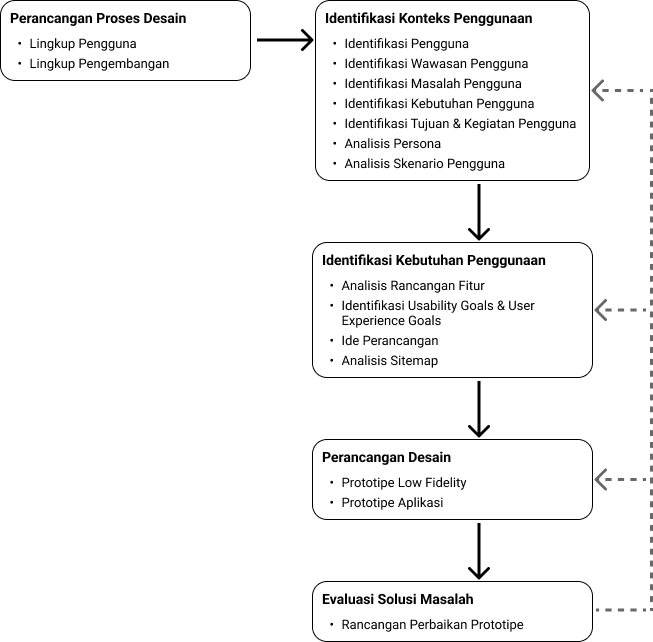
\includegraphics[width=0.8\textwidth]{chapter-3-alur-penelitian.png}
%   \caption{Alur Kerja Penelitian}
%   \label{fig:diagram_alur_kerja}
% \end{figure}

% \subsection{Perancangan Proses Desain}
% Ruang lingkup yang ditentukan pada penelitian ini adalah sebagai berikut

% \begin{enumerate}
%   \item Lingkup Pengguna
%   \subitem Target pengguna dari penelitian ini adalah masyarakat Indonesia yang pernah menggunakan atau memiliki ketertarikan terhadap aplikasi pencegah distraksi. Rentang usia dari target pengguna tidak dibatasi, namun difokuskan kepada golongan \textit{millenials} dengan rentang usia 18-30 tahun.
%   \item Lingkup Pengembangan
%   \subitem Desain interaksi aplikasi pencegah distraksi yang dibuat memiliki bentuk \textit{mobile interface} dengan mewujudkan sebuah prototipe aplikasi dalam \textit{platform Android}. Aplikasi Digital Wellbeing milik Google ditetapkan menjadi garis dasar pengembangan prototipe aplikasi tersebut.
% \end{enumerate}


% \subsection{Identifikasi Konteks Penggunaan}

% Pada tahap ini dilakukan analisis hasil riset penggunaanalisis terhadap hasil riset yang


% \subsection{Identifikasi Kebutuhan Pengguna}


% \subsection{Perancangan Desain}


% \subsection{Evaluasi Solusi Masalah}



% % Ketiga solusi yang telah diuraikan pada subbab \ref{sec:analisis_solusi} akan diimplementasikan dalam prototipe aplikasi, beserta fitur-fitur lain pada Digital Wellbeing yang akan mendukung solusi tersebut. Prototipe aplikasi ini akan diimpementasikan pada \textit{platform} Android. Secara garis besar, proses perancangan prototipe aplikasi akan menggunakan pendekatan \textit{user-centered design} (UCD).

% Seperti yang telah disebutkan pada subbab \ref{sec:metodologi}, metodologi yang digunakan dalam pengerjaan Tugas Akhir ini akan menggunakan pendekatan UCD. Dengan maksud mengikuti prosesnya, maka langkah selanjutnya yang akan dilakukan adalah mengumpulkan data. Pengumpulan data akan dilakukan dengan menyebarkan form secara online serta melakukan wawancara dengan responden yang bersedia untuk bekerja sama lebih lanjut. Proses ini akan dilaksanakan pada periode pengerjaan Tugas Akhir 2. Pengumpulan data ini bertujuan untuk melakukan validasi terhadap permasalahan yang sudah dianalisis, dan juga tidak menutup kemungkinan untuk menemukan permasalahan desain interaksi lain dari masukan pengguna.

% Setelah melakukan pengumpulan data, akan dilakukan analisis terhadap masukan yang didapat untuk mejadi kebutuhan perangkat lunak. Hasil analisis juga akan memvalidasi analisis masalah dan solusi yang didapat dari observasi penulis pada subbab \ref{sec:analisis_masalah} dan \ref{sec:analisis_solusi}.

% Kebutuhan perangkat lunak yang telah disusun akan diimplementasi dalam bentuk prototipe \textit{low-fidelity} terlebih dahulu. Setelah dilakukan evaluasi, maka implementasi akan dilanjutkan dalam bentuk prototipe \textit{high-fidelity}. Setelah menjalani evaluasi, maka perancangan prototipe aplikasi akan dikerjakan. Prototipe aplikasi diharapkan akan menghasilkan data dengan kualitas yang lebih tinggi pada saat evaluasi dibandingkan saat menggunakan prototipe \textit{low-fidelity} atau \textit{high-fidelity}. Hasil evaluasi juga akan menentukan apakah aplikasi akan menjalani proses iterasi atau diimplementasi lebih lanjut.

% \blindtext